\documentclass[12pt,a4paper]{article}
\usepackage{ctex}
\usepackage{amsmath,amscd,amsbsy,amssymb,latexsym,url,bm,amsthm}
\usepackage{epsfig,graphicx,subfigure}
\usepackage{enumitem,balance}
\usepackage{wrapfig}
\usepackage{mathrsfs,euscript}
\usepackage[usenames]{xcolor}
\usepackage{hyperref}
\usepackage[vlined,ruled,linesnumbered]{algorithm2e}
\usepackage{array}
\hypersetup{colorlinks=true,linkcolor=black}

\usepackage{pgf}
\usepackage{tikz}
\usetikzlibrary{arrows,automata}
\usepackage[latin1]{inputenc}
\newtheorem{theorem}{Theorem}
\newtheorem{lemma}[theorem]{Lemma}
\newtheorem{proposition}[theorem]{Proposition}
\newtheorem{corollary}[theorem]{Corollary}
\newtheorem{exercise}{Exercise}
\newtheorem*{solution}{Solution}
\newtheorem{definition}{Definition}
\theoremstyle{definition}

\renewcommand{\thefootnote}{\fnsymbol{footnote}}

\newcommand{\postscript}[2]
 {\setlength{\epsfxsize}{#2\hsize}
  \centerline{\epsfbox{#1}}}

\renewcommand{\baselinestretch}{1.0}

\setlength{\oddsidemargin}{-0.365in}
\setlength{\evensidemargin}{-0.365in}
\setlength{\topmargin}{-0.3in}
\setlength{\headheight}{0in}
\setlength{\headsep}{0in}
\setlength{\textheight}{10.1in}
\setlength{\textwidth}{7in}
\makeatletter \renewenvironment{proof}[1][Proof] {\par\pushQED{\qed}\normalfont\topsep6\p@\@plus6\p@\relax\trivlist\item[\hskip\labelsep\bfseries#1\@addpunct{.}]\ignorespaces}{\popQED\endtrivlist\@endpefalse} \makeatother
\makeatletter
\renewenvironment{solution}[1][Solution] {\par\pushQED{\qed}\normalfont\topsep6\p@\@plus6\p@\relax\trivlist\item[\hskip\labelsep\bfseries#1\@addpunct{.}]\ignorespaces}{\popQED\endtrivlist\@endpefalse} \makeatother

\begin{document}
\noindent

%========================================================================
\noindent\framebox[\linewidth]{\shortstack[c]{
\Large{\textbf{Lab10-Turing Machine}}\vspace{1mm}\\
CS214-Algorithm and Complexity, Xiaofeng Gao \& Lei Wang, Spring 2021.}}
\begin{center}
\footnotesize{\color{red}$*$ If there is any problem, please contact TA Yihao Xie. }

\footnotesize{\color{blue}$*$ Name:Yanjie Ze  \quad Student ID:519021910706 \quad Email: zeyanjie@sjtu.edu.cn}
\end{center}

\begin{enumerate}
    \item Design a one-tape TM $M$ that computes the function $f(x, y) = \lfloor x/y \rfloor$, where $x$ and $y$ are positive integers $(x > y)$. The alphabet is $\{1, 0, \Box, \triangleright, \triangleleft\}$, and the inputs are $x$ "1"s, $\Box$ and $y$ "1"s. Below is the initial configuration for input $x=7$ and $y=3$. The result $z=f(x,y)$ should also be represented in the form of $z$ "1"s on the tape with pattern of $\rhd 111\cdots 111\lhd$, which is $\rhd 11\lhd$ for the example.
    
	\begin{center}
		\begin{tabular}{ll|c|c|c|c|c|c|c|c|c|c|c|c|c|c}
			& \multicolumn{14}{c}{Initial Configuration}\\[5pt]
			\cline{2-16}
			& & $\triangleright$ &  1  & 1 & 1 & 1 & 1 & 1 & 1 & $\Box$ & 1 & 1 & 1 & $ \triangleleft$ & \\
			\cline{2-16}
			\multicolumn{2}{c}{} & \multicolumn{1}{c}{$\uparrow$} & \multicolumn{11}{c}{}\\[-4pt]
			\multicolumn{2}{c}{} & \multicolumn{1}{c}{$q_S$} & \multicolumn{11}{c}{}	
		\end{tabular}
	\end{center}

    \begin{enumerate}
	\item
	Please describe your design and then write the specifications of $M$ in the form like $\langle q_S, \triangleright \rangle \rightarrow \langle q_1, \triangleright,  R\rangle$. Explain the transition functions in detail.
	\begin{solution}
	~\\
	\textbf{Set of States}:
	$$
	Q=\{q_S, q_Y, q_{CY}, q_{CX}, q_R,q_W,q_{WW},q_F,q_{FF},q_{FFF}, q_H\}
	$$
	The meanings of the states are shown in the following table.
	
	\begin{center}
	\begin{tabular}{c|c}
	\hline
	state & meaning\\
	\hline
	   $q_S$  &  the start state\\
	   $q_Y$  & the reading head goes to $y$\\
	   $q_{CY}$ & the reading head does comparison in $y$\\
	   $q_{CX}$ &the reading head does comparison in $x$ \\ 
	   $q_W$ &recovering 1 in $y$ \\
	   $q_{WW}$ &recovering 1 in $y$ and avoiding entering $x$ \\
	   $q_R$ & writing 1 to the result\\
	   $q_F$ & the final state at $x$\\
	   $q_{FF}$ & the final state at $y$ \\
	   $q_{FFF}$ & the final state in the output tape\\
	   $q_H$ & the end state \\
	   \hline
	\end{tabular}
		\end{center}
	
	\textbf{Transition Functions}:	
	\begin{enumerate}
	
	    \item Go to find the start of y:
	    $$
	    \langle q_S, \triangleright \rangle \rightarrow \langle q_Y,\triangleright, R \rangle
	    $$
	     $$
	    \langle q_Y, 1 \rangle \rightarrow \langle q_Y,1, R \rangle
	    $$
	    $$
	    \langle q_Y, 0 \rangle \rightarrow \langle q_Y,0, R \rangle
	    $$
	    $$
	     \langle q_Y, \Box \rangle \rightarrow \langle q_{CY},\Box, R \rangle
	    $$
	    \item Begin to compare the number of 1 in $x$ and $y$. 
	    \begin{enumerate}
	        \item Find 1 in $y$ and transform it into 0, to represent it has been read. Once we find a 1, we begin to move left.
	    
	        $$
	         \langle q_{CY}, 0 \rangle \rightarrow \langle q_{CY},0, R \rangle
	        $$
	        $$
	         \langle q_{CY}, 1 \rangle \rightarrow \langle q_{X},0, L \rangle
	        $$
	        
	       \item The reading head needs to move to the position of $x$.
	       $$
	         \langle q_{X}, \Box \rangle \rightarrow \langle q_{CX},\Box, S \rangle
	        $$
	        $$
	         \langle q_{X}, 0 \rangle \rightarrow \langle q_X,0, L \rangle
	        $$
	         $$
	         \langle q_{X}, 1 \rangle \rightarrow \langle q_X,1, L \rangle
	        $$
	      \item Find  1 in $x$ and transform it into 0, to represent it has been read. Once we find a 1, we begin to move right.
	       $$
	         \langle q_{CX}, \Box \rangle \rightarrow \langle q_{CX},\Box, L \rangle
	        $$
	      $$
	         \langle q_{CX}, 1 \rangle \rightarrow \langle q_{Y},0, R \rangle
	        $$
	        $$
	         \langle q_{CX}, 0 \rangle \rightarrow \langle q_{CX},0, L \rangle
	        $$
	     
	       \item Once all ones in $y$ have been transformed into 0, and the reading head reaches $\triangleleft$, we can \textbf{add 1 to the result}. We first transform $\triangleleft$ to $\Box$ then write results behind $\Box$.
	       $$
	       \langle q_{CY},\triangleleft \rangle \rightarrow \langle q_{R}, \Box, R\rangle
	       $$
	       $$
	       \langle q_{CY},\Box \rangle \rightarrow \langle q_{R}, \Box, R\rangle
	       $$
	       $$
	       \langle q_{R},\Box \rangle \rightarrow \langle q_{W}, 1, L\rangle
	       $$
	       $$
	       \langle q_{R},1 \rangle \rightarrow \langle q_{R}, 1, R\rangle
	       $$
	       \item After writing one result, we need to recover all ones in $y$, because they are currently 0. We first move the reading head back and then begin to write.
	        $$
	       \langle q_{W},0 \rangle \rightarrow \langle q_{W}, 0, L\rangle
	       $$
	       $$
	       \langle q_{W},1 \rangle \rightarrow \langle q_{W}, 1, L\rangle
	       $$
	       $$
	       \langle q_{W},\Box \rangle \rightarrow \langle q_{WW}, \Box, L\rangle
	       $$
	       $$
	       \langle q_{WW},0 \rangle \rightarrow \langle q_{WW}, 1, L\rangle
	       $$
	        $$
	       \langle q_{WW},1 \rangle \rightarrow \langle q_{WW}, 1, L\rangle
	       $$
	        $$
	       \langle q_{WW},\Box \rangle \rightarrow \langle q_{CY}, \Box, S\rangle
	       $$
	       
	       
	          \item If we successfully transform 1 in $y$ to 0 but fail to find a corresponding 1 in $x$, the reading head will reach $\triangleright$, this means the result is determined. All 1 for the result has been written.
	           $$
	       \langle q_{CX},\triangleright \rangle \rightarrow \langle q_{F}, \triangleright, R\rangle
	       $$
	       $$
	       \langle q_{F},0 \rangle \rightarrow \langle q_{F}, 0, R\rangle
	       $$
	       $$
	       \langle q_{F},\Box \rangle \rightarrow \langle q_{FF}, \Box, R\rangle
	       $$
	        $$
	       \langle q_{FF},0 \rangle \rightarrow \langle q_{FF}, 0, R\rangle
	       $$
	       $$
	       \langle q_{FF},1 \rangle \rightarrow \langle q_{FF}, 1, R\rangle
	       $$
	       $$
	       \langle q_{FF},\Box \rangle \rightarrow \langle q_{FFF}, \Box, R\rangle
	       $$
	       $$
	       \langle q_{FF},\triangleleft \rangle \rightarrow \langle q_{FFF}, \triangleleft, S\rangle\quad(special\ case\ for\ no\ 1\ in\ output)
	       $$
	       $$
	       \langle q_{FFF},1 \rangle \rightarrow \langle q_{FFF}, 1, R\rangle
	       $$
	       $$
	       \langle q_{FFF},\Box \rangle \rightarrow \langle q_{FFF}, \triangleleft , S\rangle
	       \quad (write\ the\ end\ symbol)$$
	       
	     \item The exit state:
	     $$
	        \langle q_{FFF},\triangleleft \rangle \rightarrow \langle q_{H}, \triangleleft , S\rangle 
	       $$
	       
	    \end{enumerate}
	    
	    
	\end{enumerate}
	\end{solution}
	\item
	Please draw the state transition diagram.
	
\begin{tikzpicture}[->,>=stealth',shorten >=1pt,auto,node distance=5.2cm,
                    thick]
  \tikzstyle{every state}=[fill=red!5,draw=red!60,text=black]

  \node[initial,state] (S)                    {$q_S$};
  \node[accepting,state]         (Y) [right  of=S] {$q_Y$};
    \node[accepting,state]         (CY) [below right of=Y] {$q_{CY}$};
  \node[accepting,state]         (X) [below left of=CY] {$q_X$};

  \node[accepting,state]         (CX) [below left of=Y]       {$q_{CX}$};
    \node[accepting,state]         (R) [below  of=CY]       {$q_{R}$};
  \node[accepting,state]         (W) [below  of=R]       {$q_{W}$};
  \node[accepting,state]         (WW) [below right of=W]       {$q_{WW}$};

  \node[accepting,state]         (F) [below  of=CX]       {$q_{F}$};
  \node[accepting,state]         (FF) [below  of=F]       {$q_{FF}$};
  \node[accepting,state]         (FFF) [below of=FF]       {$q_{FFF}$};
    \node[accepting,state]         (H) [right of=FFF]       {$q_{H}$};

  

  \path (S) edge node {$\triangleright, \triangleright ,R$ } (Y)
       (Y) edge   [loop below]           node {1,1,R} (Y)
(Y) edge     [loop right]         node {0,0,R} (Y)
(Y) edge              node {$\Box,\Box,R$} (CY)
(CY) edge    [loop left]          node {0,0,R} (CY)
(CY) edge              node {1,0,L} (X)
(X) edge              node {$\Box,\Box,S$} (CX)
(X) edge     [loop below]         node {0,0,L} (X)
(X) edge     [loop right]         node {1,1,L} (X)
(CX) edge   [loop right]           node {$\Box,\Box,L$} (CX)
(CX) edge              node {1,0,R} (Y)
(CX) edge    [loop left]          node {0,0,L} (CX)
(CY) edge      [bend left]        node {$\triangleleft,\Box,R$} (R)
(CY) edge    [bend right]          node {$\Box,\Box,R$} (R)
(R) edge              node {$\Box,1,L$} (W)
(R) edge     [loop right]         node {1,1,R} (R)
(W) edge    [loop right]          node {1,1,L} (W)
(W) edge    [loop left]          node {0,1,L} (W)
(W) edge              node {$\Box,\Box,L$} (WW)
(WW) edge      [loop left]        node {0,1,L} (WW)
(WW) edge       [loop right]       node {1,1,L} (WW)
(WW) edge      [bend right]        node {$\Box,\Box,R$} (CY)
(CX) edge      [bend right]        node {$\triangleright,\triangleright,R$} (F)
(F) edge     [loop right]         node {0,0,R} (F)
(F) edge          node {$\Box,\Box,R$} (FF)
(FF) edge     [loop right]         node {0,0,R} (FF)
(FF) edge     [loop left]         node {1,1,R} (FF)
(FF) edge      [bend right]        node {$\Box,\Box,R$} (FFF)
(FF) edge     [bend left]         node {$\triangleleft,\triangleleft,S$} (FFF)
(FFF) edge      [loop below]        node {1,1,R} (FFF)
(FFF) edge      [loop left]        node {$\Box,\triangleleft,S$} (FFF)
(FFF) edge        node {$\triangleleft,\triangleleft,S$} (H);

        
        
\end{tikzpicture}
	\item
	Show briefly and clearly the whole process from initial to final configurations for input $x = 7$ and $y = 3$. You may start like this:
	$$(q_s,\underline{\triangleright}  1  1  1  1  1  1  1  \Box 1  1  1   \triangleleft)
	\vdash (q_1,\triangleright  \underline{1}  1  1  1  1  1  1  \Box 1  1  1   \triangleleft)
	\vdash^* (q_1,\triangleright  1  1  1  1  1  1  1  \underline{\Box} 1  1  1   \triangleleft)
	\vdash (q_2,\triangleright  1  1  1  1  1  1  1  \Box \underline{1}  1  1   \triangleleft)$$
	
	\par{\color{blue}(Note that for simplicity, we write $(q_1,\triangleright  \underline{1}  1  1  1  1  1  1  \Box 1  1  1   \triangleleft)\vdash^* (q_1,\triangleright  1  1  1  1  1  1  1  \underline{\Box} 1  1  1   \triangleleft)$ if the corresponding transaction repeats on multiple inputs with the same state.)}
	\begin{solution}
	$$
	(q_S,\underline{\triangleright}  1  1  1  1  1  1  1  \Box 1  1  1   \triangleleft)
	$$
	$$
	\vdash(q_Y,\triangleright  \underline{1}  1  1  1  1  1  1  \Box 1  1  1   \triangleleft)
	$$
	$$
	\vdash^*(q_Y,\triangleright  1  1  1  1  1  1  1  \underline{\Box} 1  1  1   \triangleleft)
	$$
	$$
	\vdash(q_{CY},\triangleright  1  1  1  1  1  1  1  \Box \underline{0}  1  1   \triangleleft)
	$$
	$$
	\vdash(q_X,\triangleright  1  1  1  1  1  1  1  \underline{\Box} 0  1  1   \triangleleft)
	$$
	$$
	\vdash(q_{CX},\triangleright  1  1  1  1  1  1  \underline{0}  \Box 0  1  1   \triangleleft)
	$$
	$$
	\vdash(q_{Y},\triangleright  1  1  1  1  1  1  0  \underline{\Box} 0  1  1   \triangleleft)
	$$
	$$
	\vdash(q_{CY},\triangleright  1  1  1  1  1  1  0  \Box \underline{0}  1  1   \triangleleft)
	$$
	$$
	\vdash(q_{CY},\triangleright  1  1  1  1  1  1  0  \Box 0  \underline{0}  1   \triangleleft)
	$$
	$$
	\vdash(q_{X},\triangleright  1  1  1  1  1  1  0  \Box \underline{0}  0  1   \triangleleft)
	$$
	$$
	\vdash(q_{X},\triangleright  1  1  1  1  1  1  0  \underline{\Box} 0  0  1   \triangleleft)
	$$
		$$
	\vdash(q_{CX},\triangleright  1  1  1  1  1  1  \underline{0}  \Box 0  0  1   \triangleleft)
	$$
		$$
	\vdash(q_{CX},\triangleright  1  1  1  1  1  \underline{0}  0  \Box 0  0  1   \triangleleft)
	$$
		$$
	\vdash(q_{Y},\triangleright  1  1  1  1  1  0  \underline{0}  \Box 0  0  1   \triangleleft)
	$$
	$$
	\vdash(q_{Y},\triangleright  1  1  1  1  1  0  0  \underline{\Box} 0  0  1   \triangleleft)
	$$
	$$
	\vdash(q_{CY},\triangleright  1  1  1  1  1  0  0  \Box \underline{0}  0  1  \triangleleft)
	$$
	$$
	\vdash^*(q_{CY},\triangleright  1  1  1  1  1  0  0  \Box 0  0  \underline{0}   \triangleleft)
	$$
	$$
	\vdash(q_{X},\triangleright  1  1  1  1  1  0  0  \Box 0  \underline{0}  0   \triangleleft)
	$$
	$$
	\vdash^*(q_{X},\triangleright  1  1  1  1  1  0  0  \underline{\Box} 0  0  0   \triangleleft)
	$$
	$$
	\vdash(q_{CX},\triangleright  1  1  1  1  1  0  \underline{0}  \Box 0  0  0   \triangleleft)
	$$
	$$
	\vdash^*(q_{CX},\triangleright  1  1  1  1  \underline{0}  0  0  \Box 0  0  0   \triangleleft)
	$$
	$$
	\vdash(q_{Y},\triangleright  1  1  1  1  0  \underline{0}  0  \Box 0  0  0   \triangleleft)
	$$
	$$
	\vdash^*(q_{Y},\triangleright  1  1  1  1  0  0  0  \underline{\Box} 0  0  0   \triangleleft)
	$$
	$$
	\vdash(q_{CY},\triangleright  1  1  1  1  0  0  0  \Box \underline{0}  0  0   \triangleleft)
	$$
	$$
	\vdash^*(q_{CY},\triangleright  1  1  1  1  0  0  0  \Box 0  0  0   \underline{\Box} \Box)
	$$
	$$
	\vdash(q_{R},\triangleright  1  1  1  1  0  0  0  \Box 0  0  0  \Box \underline{1})
	$$
	$$
	\vdash(q_{W},\triangleright  1  1  1  1  0  0  0  \Box 0  0  0  \underline{\Box} 1)
	$$
	$$
	\vdash(q_{WW},\triangleright  1  1  1  1  0  0  0  \Box 0  0  \underline{1}  \Box 1)
	$$
	$$
	\vdash(q_{WW},\triangleright  1  1  1  1  0  0  0  \Box 0  \underline{1}  1  \Box 1)
	$$
	$$
	\vdash(q_{WW},\triangleright  1  1  1  1  0  0  0  \Box \underline{1}  1  1  \Box 1)
	$$
	$$
	\vdash(q_{WW},\triangleright  1  1  1  1  0  0  0  \underline{\Box} 1  1  1  \Box 1)
	$$
	$$
	\vdash(q_{CY},\triangleright  1  1  1  1  0  0  0  \Box \underline{1} 1  1  \Box 1)
	$$
	 We repeat the same process to get another 1, and we will get:
	$$
    (q_{CY},\triangleright  1  0  0  0  0  0  0  \Box \underline{0}  1  1  \Box 1 1)
	$$
	Then we continue showing the remaining process:
	$$
    \vdash(q_{X},\triangleright  1  0  0  0  0  0  0  \underline{\Box} 0  1  1  \Box 1 1)
	$$
	$$
    \vdash(q_{CX},\triangleright  1  0  0  0  0  0  0  \Box 0  1  1  \Box 1 1)
	$$
	$$
    \vdash^*(q_{CX},\triangleright  \underline{0}  0  0  0  0  0  0  \Box 0  1  1  \Box 1 1)
	$$
	$$
    \vdash(q_{Y},\triangleright  0  \underline{0}  0  0  0  0  0  \Box 0  1  1  \Box 1 1)
	$$
	$$
    \vdash^*(q_{Y},\triangleright  0  0  0  0  0  0  0  \underline{\Box} 0  1  1  \Box 1 1)
	$$
	$$
    \vdash(q_{CY},\triangleright  0  0  0  0  0  0  0  \Box \underline{0}  1  1  \Box 1 1)
	$$
	$$
    \vdash(q_{CY},\triangleright  0  0  0  0  0  0  0  \Box 0  \underline{0}  1  \Box 1 1)
	$$
	$$
    \vdash(q_{X},\triangleright  0  0  0  0  0  0  0  \Box \underline{0}  0  1  \Box 1 1)
	$$
	$$
    \vdash(q_{X},\triangleright  0  0  0  0  0  0  0  \underline{\Box} 0  0  1  \Box 1 1)
	$$
	$$
    \vdash(q_{CX},\triangleright  0  0  0  0  0  0  \underline{0}  \Box 0  0  1  \Box 1 1)
	$$
	$$
    \vdash^*(q_{CX},\underline{\triangleright}  0  0  0  0  0  0  0  \Box 0  0  1  \Box 1 1)
	$$
	$$
    \vdash(q_{F},\triangleright  \underline{0}  0  0  0  0  0  0  \Box 0  0  1  \Box 1 1)
	$$
	$$
    \vdash^*(q_{F},\triangleright  0  0  0  0  0  0  0  \underline{\Box} 0  0  1  \Box 1 1)
	$$
	$$
    \vdash(q_{FF},\triangleright  0  0  0  0  0  0  0  \Box \underline{0}  0  1  \Box 1 1)
	$$
	$$
    \vdash^*(q_{FF},\triangleright  0  0  0  0  0  0  0  \Box 0  0  1 \underline{\Box} 1 1)
	$$
	$$
    \vdash(q_{FFF},\triangleright  0  0  0  0  0  0  0  \Box 0  0  1  \Box \underline{1} 1)
	$$
	$$
    \vdash(q_{FFF},\triangleright  0  0  0  0  0  0  0  \Box 0  0  1  \Box 1 \underline{1} \Box)
	$$
	$$
    \vdash(q_{FFF},\triangleright  0  0  0  0  0  0  0  \Box 0  0  1  \Box 1 1 \underline{\triangleleft})
	$$
	$$
    \vdash(q_{H},\triangleright  0  0  0  0  0  0  0  \Box 0  0  1  \Box 1 1 \underline{\triangleleft})
	$$
	We reach the final state, and the number of ones behind the second square $\Box$ is the result, which is $\lfloor 7/3\rfloor=2$.
	\end{solution}
	
\end{enumerate}

    \item 
    Given the alphabet $\{1, 0, \Box, \triangleright, \triangleleft\}$, design a time efficient 3-tape TM $M$ to compute $f:\{0,1\}^*\rightarrow\{0,1\}$ which verifies whether the number of 0 and the number of 1 are the same in an input consisting of only 0's and 1's. $M$ should output 1 if the numbers are the same, and 0 otherwise. For eample, for the input tape $\triangleright 001101\triangleleft$, $M$ should output 1.
    
    \begin{enumerate}
	    \item
	    Please describe your design and then write the specifications of $M$ in the form like $\langle q_S, \triangleright, \triangleright \rangle \rightarrow \langle q_1, \triangleright,  R, R \rangle$. Explain the transition functions in detail.
	    \begin{solution}
	    ~\\
	   \textbf{ The whole process of our turing machine is}:
	    \begin{enumerate}
	        \item Read every element one by one on the first tape. When the reading head reads $0$, it copies $0$ to the second tape.
	        \item After finishing reading the input, the reading head on the first tape and the reading head on the second tape begin to scan back.
	        \begin{itemize}
	            \item If the first reading head encounters $0$, it skips and scans next element. 
	            \item If the first reading head encounters $1$, and at this time the second reading head check whether there exists $0$. If there exists corresponding $0$, both reading heads will go to scan next element. If there doesn't exist corresponding $0$, TM outputs $0$ on the third tape.
	            \item If the first reading head has finished scanning but the second tape hasn't, TM outputs $0$ on the third tape.
	        \end{itemize}
	        \item After both reading heads finish scanning back and the third tape still has no output, this means the number of 0 and the number of 1 are the same.
	    \end{enumerate}
	    
	    ~\\
	    \textbf{Set of states:}
	    $$
	    Q=\{q_S,q_C,q_R, q_T\}
	    $$
	    Where $q_S$ means the start state, $q_C$ means the copying state, $q_R$ means the comparing state and $q_T$ means the termination state.
	    
	    ~\\
	    \textbf{Transition functions:}
	    
	    \begin{enumerate}
	        \item Start State:
	        $$
	        \langle q_S, \triangleright, \triangleright,\triangleright \rangle \rightarrow \langle q_C,\triangleright,\triangleright,R,R,R \rangle
	        $$
	        \item Begin to copy:
	        \begin{itemize}
	        \item 1st tape reads $0$ and moves. 2nd tape copies $0$ and moves. 3rd tape stays:
	        $$
	        \langle q_C,0,\Box,\Box  \rangle \rightarrow \langle q_C,0,\Box,R,R,S \rangle
	        $$
	        \item 1st tape reads $1$ and moves. 2nd tape does no copy and stays. 3rd tape stays:
	        $$
	        \langle q_C,1,\Box,\Box  \rangle \rightarrow \langle q_C,\Box,\Box,R,S,S \rangle
	        $$
	        \item 1st tape reads $\triangleleft$ and moves back. 2nd tape moves back. 3rd tape stays:
	        $$
	        \langle q_C,\triangleleft,\Box,\Box  \rangle \rightarrow \langle q_R,\Box,\Box,L,L,S \rangle
	        $$
	        \end{itemize}
	        \item Begin to compare:
	        \begin{itemize}
	            \item 1st tape reads 1 and 2nd tape reads 0, which is one match. Two tapes moves back. 3rd tape stays:
	            $$
	        \langle q_R,1,0,\Box  \rangle \rightarrow \langle q_R,0,\Box,L,L,S \rangle
	        $$
	        \item 1st tape reads 0 and 2nd tape reads 0. 1st tape skips this 0 and moves back. Another two tapes stay:
	         $$
	        \langle q_R,0,0,\Box  \rangle \rightarrow \langle q_R,0,\Box,L,S,S \rangle
	        $$
	        \item 1st tape reads 0 and 2nd tape reaches the head. 1st tape continues to move back:
	         $$
	        \langle q_R,0,\triangleright,\Box  \rangle \rightarrow \langle q_R,\triangleright,\Box,L,S,S \rangle
	        $$
	        \item 1st tape reads $1$ and 2nd tape reaches the head. This means the number of 0 and the number of 1 are different. TM output 0:
	         $$
	        \langle q_R,1,\triangleright,\Box  \rangle \rightarrow \langle q_T,\triangleright,0,S,S,S \rangle
	        $$
	        \item Both 1st tape and 2nd tape reach the head. This means the number of 0 and the number of 1 are the same. TM output 1:
	         $$
	        \langle q_R,\triangleright,\triangleright,\Box  \rangle \rightarrow \langle q_T,\triangleright,1,S,S,S \rangle
	        $$
	        \item 1st tape reaches the head and 2nd tape reads 0. This means the number of 0 and the number of 1 are different. TM outputs 0:
	        $$
	        \langle q_R,\triangleright,0,\Box  \rangle \rightarrow \langle q_T,0,0,S,S,S \rangle
	        $$
	        \end{itemize}
	    \end{enumerate}
	    \end{solution}
	    \item 
	    Show the time complexity for one-tape TM $M'$ to compute the same function $f$ with $n$ symbols in the input and give a brief description of such $M'$ .
	    \begin{solution}
	    ~\\
	    We assume there are $m$ zeros in the input. $m$ satisfies $0\leq m \leq n$.
	    
	    We take the input as $\mathbf{0101101}$ for an example.
	    ~\\
	    \textbf{The outline of the algorithm:} 
	    
	    \begin{enumerate}
	        \item The reading head starts to copy all zeros to $n+1,n+2,...,n+m$ positions. We use $\Box$ to divide the origin and the copy.
	        
	        The cost of copying is:
	        $$
	        T_{copy} = (n+1)+(n+2)+...+(n+m)=mn+\frac{m^2+m}{2}
	        $$
	       
	        \item The reading head begins to compare the copy and the origin. Staring from $\triangleright$:
	        \begin{enumerate}
	            \item The reading head reads one zero in the copy and transform it into $\Box$. Then the reading head moves to the origin. 
	            \item If the reading head reads 1 in the origin first, this means one match. Transform it into $\Box$. Then the reading head moves back to the copy.
	            \item If the reading head reads 0 in the origin first, it needs to skip this to find 1. Transform 1 into $\Box$ and scan next.
              
	        \end{enumerate}
	        \item The termintion condition is:
	        \begin{enumerate}
	             \item If all the zeros in the copy have been replaced  but the reading head still finds 1 in the origin, TM outputs 0.
                \item If all the ones in the origin have been replaced but the reading head still finds 0 in the copy, TM outputs 0.
                \item If all the elements in the type have become $\Box$ and TM has no output yet, TM outputs 1.
	        \end{enumerate}
	        \end{enumerate}
	   Here is one example of inputing $\mathbf{0101101}$. TM outputs 0.
	
	        	\begin{center}
		\begin{tabular}{ll|c|c|c|c|c|c|c|c|c|c|c|c|c|c}
			& \multicolumn{14}{c}{After Finishing Copying}\\[5pt]
			\cline{2-16}
			& & $\triangleright$ &  0  & 1 & 0 & 1 & 1 & 0 & 1 & $\Box$ & 0 & 0 & 0 & $ \triangleleft$ & \\
			\cline{2-16}
			\multicolumn{2}{c}{} & \multicolumn{1}{c}{} & \multicolumn{11}{c}{}\\[-4pt]
			\multicolumn{2}{c}{} & \multicolumn{1}{c}{} & \multicolumn{11}{c}{}	
		\end{tabular}
	\end{center}
	        \begin{center}
		\begin{tabular}{ll|c|c|c|c|c|c|c|c|c|c|c|c|c|c}
			& \multicolumn{14}{c}{After One Comparison}\\[5pt]
			\cline{2-16}
			& & $\triangleright$ &  0  & 1 & 0 & 1 & 1 & 0 & $\Box$ & $\Box$ & 0 & 0 & $\Box$ & $ \triangleleft$ & \\
			\cline{2-16}
			\multicolumn{2}{c}{} & \multicolumn{1}{c}{} & \multicolumn{11}{c}{}\\[-4pt]
			\multicolumn{2}{c}{} & \multicolumn{1}{c}{} & \multicolumn{11}{c}{}	
		\end{tabular}
	\end{center}
	\begin{center}
		\begin{tabular}{ll|c|c|c|c|c|c|c|c|c|c|c|c|c|c}
			& \multicolumn{14}{c}{After Two Comparisons}\\[5pt]
			\cline{2-16}
			& & $\triangleright$ &  0  & 1 & 0 & 1 & $\Box$ & $\Box$ & $\Box$ & $\Box$ & 0 & $\Box$ & $\Box$ & $ \triangleleft$ & \\
			\cline{2-16}
			\multicolumn{2}{c}{} & \multicolumn{1}{c}{} & \multicolumn{11}{c}{}\\[-4pt]
			\multicolumn{2}{c}{} & \multicolumn{1}{c}{} & \multicolumn{11}{c}{}	
		\end{tabular}
	\end{center}
	
		\begin{center}
		\begin{tabular}{ll|c|c|c|c|c|c|c|c|c|c|c|c|c|c}
			& \multicolumn{14}{c}{After Three Comparisons, Output $\mathbf{0}$ }\\[5pt]
			\cline{2-16}
			& & $\triangleright$ &  0  & 1 & 0 & $\Box$ & $\Box$ & $\Box$ & $\Box$ & $\Box$ & $\Box$ & $\Box$ & $\Box$ & $ \triangleleft$ & \\
			\cline{2-16}
			\multicolumn{2}{c}{} & \multicolumn{1}{c}{} & \multicolumn{11}{c}{}\\[-4pt]
			\multicolumn{2}{c}{} & \multicolumn{1}{c}{} & \multicolumn{11}{c}{}	
		\end{tabular}
	\end{center}
	    
	  The cost of comparison is:
	  $$
	  T_{comp} = O(m+n)\times m = O(m^2+mn)
	  $$
	  The total cost is:
	  $$
	  T_{total}=T_{copy}+T_{comp}=mn+\frac{m^2+m}{2} + O(m^2+mn) =O(m^2+mn)
	  $$
	  Since $0\leq m\leq n$, we have:
	  $$
	  T_{total} = O(n^2)
	  $$
	    \end{solution}
	
	\end{enumerate}
	
	\item Define the corresponding decision or search problem of the following problems and give the "certificate" and "certifier" for each decision problem provided in the subquestions or defined by yourself.
	
	\begin{enumerate}
	    \item
	    \textit{3-Dimensional Matching.}  Given disjoint sets $X,Y,Z$ all with the size of $n$, and a set $M \subseteq X\times Y\times Z$.  Is there a subset $M'$ of $M$ of size $n$ where no two elements of $M'$ agree in any coordinate?
	    \begin{solution}
	    ~\\
	    \textbf{Decision Problem}: Does there \textbf{exist} a subset M' of M of size n where no two elements of M' agree in any coordinate?
	    
	    \textbf{Search Problem}: Given $M\subseteq X\times Y\times Z$, \textbf{find} a subset M' of M of size n where no elements of M agree in any coordinate?
	    
	    \textbf{Certificate}: A subset M' of M of size n where no two elements agree in any coordinate
	    
	    \textbf{Certifier}: Check that M' is the subset of M and each two elements of M' don't agree in any coordinate, as shown in Alg.~\ref{cert1}.
	    
	    \begin{center}
	    \begin{algorithm}[H]
	    \caption{Certifier(M',M)}
	    \label{cert1}
	    \textbf{Input:}two set $M'$, $M$\;
	    \If{$M'$ is not the subset of $M$}
	    {
	    \Return $False$\;
	    }
	    \For{each element $a\in M'$}
        {
        \For{each element $b\in M'$}
        {\If{$a$ and $b$ are not the same element}
        {
        \If{each dimension of $a$ is different from $b$}
        {
        Continue\;}
        \Else{\Return $False$\;}
        }
        }
        }	    
	    \end{algorithm}
	    \end{center}
	    
	    \end{solution}
	    \item 
	    \textit{Travelling Salesman Problem.} Given a list of cities and the distances between each pair of cities, find the shortest possible route that visits each city exactly once and returns to the origin city.
	    \begin{solution}
	    ~\\
	    \textbf{Decision Problem}: Does there \textbf{exist} a route that
visits each city exactly once and returns to the origin city, with the length of the path  $\leqslant k$?

	    \textbf{Search Problem}: \textbf{Find} the shortest possible route that visits each city exactly once and returns to the origin city.
	    
	    \textbf{Certificate}: A path that visits each city exactly once and returns to the origin city.
	    
	    \textbf{Certifier}: Check whether the path visits each city exactly once and returns to the origin city, and the length of the path is smaller than $k$, as shown in Alg.~\ref{cert2}.
	    
	    \begin{center}
	        \begin{algorithm}[H]
	        \caption{Certifier(P, k)}
	        \textbf{Input:} path $P=\{e_1,e_2,..,e_n\}$, bound $k$\;
	        \If{Along the path $P$, there exists a city not visited or visited more than once}
	        {\Return $False$\;
	        }
	        \If{Along the path $P$, the visitor can't return to the origin city}
	        {\Return $False$\;
	        }
	        Define $sum=0$\;
	        \For{each edge $e$ in $P$}
	        {$sum += length(e)$\;
	        }
	        \If{$sum\leq k$}
	        {
	        \Return $True$\;
	        }
	        \Else{\Return $False$\;}
	        
	        \label{cert2}
	        
	        \end{algorithm}
	    \end{center}
	    
	    \end{solution}
	    \item
	    \textit{Job Sequencing.} Given a set of unit-time jobs, each of which has an integer deadline and a non-negative penalty for missing the deadline. Does there exist a job sequence that has a total penalty $w\leqslant k$?
	     \begin{solution}
	    ~\\
	    \textbf{Decision Problem}: Does there \textbf{exist} a job sequence that has a total penalty $w\leqslant k$?
	    
	    \textbf{Search Problem}: \textbf{Find} a job sequence that has a total penalty $w\leqslant k$.
	    
	   
	    
	    \textbf{Certificate}: A job sequence of unit-time jobs, each of which has an integer deadline and a non-negative penalty for missing the deadline.
	    
	    \textbf{Certifier}: Check whether the total penalty of the job sequence is smaller than $k$, as shown in Alg.~\ref{cert3}.
	    
	    \begin{center}
	        \begin{algorithm}[H]
	        \caption{Certifier(S, k)}
	        \label{cert3}
	        \textbf{Input:} job sequence $S$, bound $k$\;
	        Define $sum_p=0$ as the total penalty\;
	        \For{each job $j\in S$}
	        {\If{$j$ is finished later than the deadline}
	        {$sum_p += penalty(j) $
	        }
	        }
	        \If{$sum_p\leq k$}{\Return $True$\;}
	        \Else{\Return $False$\;}
	        
	        \end{algorithm}
	    \end{center}
	    \end{solution}
	\end{enumerate}
\end{enumerate}

\textbf{Remark:} Please include your .pdf, .tex files for uploading with standard file names.
\newpage


%========================================================================
\end{document}